\section{Introduction}
\label{sec:intro}

Feed-forward 3D foundation models have, since 2024, become the dominant way to recover geometry
from images. Where classical photogrammetry needed many overlapping photographs, careful camera
calibration, and a slow two-stage optimization (structure-from-motion for the cameras, then
multi-view stereo for dense geometry), these models regress geometry \emph{directly} from raw
pixels. DUSt3R-style models~\cite{dust3r,mast3r} predict a per-pixel \emph{point map}---for every
pixel, the $(x,y,z)$ coordinate of the surface it sees, expressed in one shared coordinate
frame---and recent transformers scale this to many views and unify depth, camera pose and point
maps in a single forward pass~\cite{vggt,fast3r,cut3r,pi3}. \vggt~\cite{vggt} won the CVPR'25 Best
Paper Award; \pii~\cite{pi3} made the architecture permutation-equivariant (its output does not
depend on the order in which the images are fed). These models are released openly, run in seconds
on a single GPU, and their entire value lies in \emph{downstream use}: multi-view fusion into a
clean point cloud, 3D Gaussian Splatting initialization~\cite{instantsplat,gsplat}, SLAM and
robotics. Every such consumer faces the same question before it can act: \emph{which of the
predicted points should it trust?}

\begin{figure*}[tbp]
  \centering
  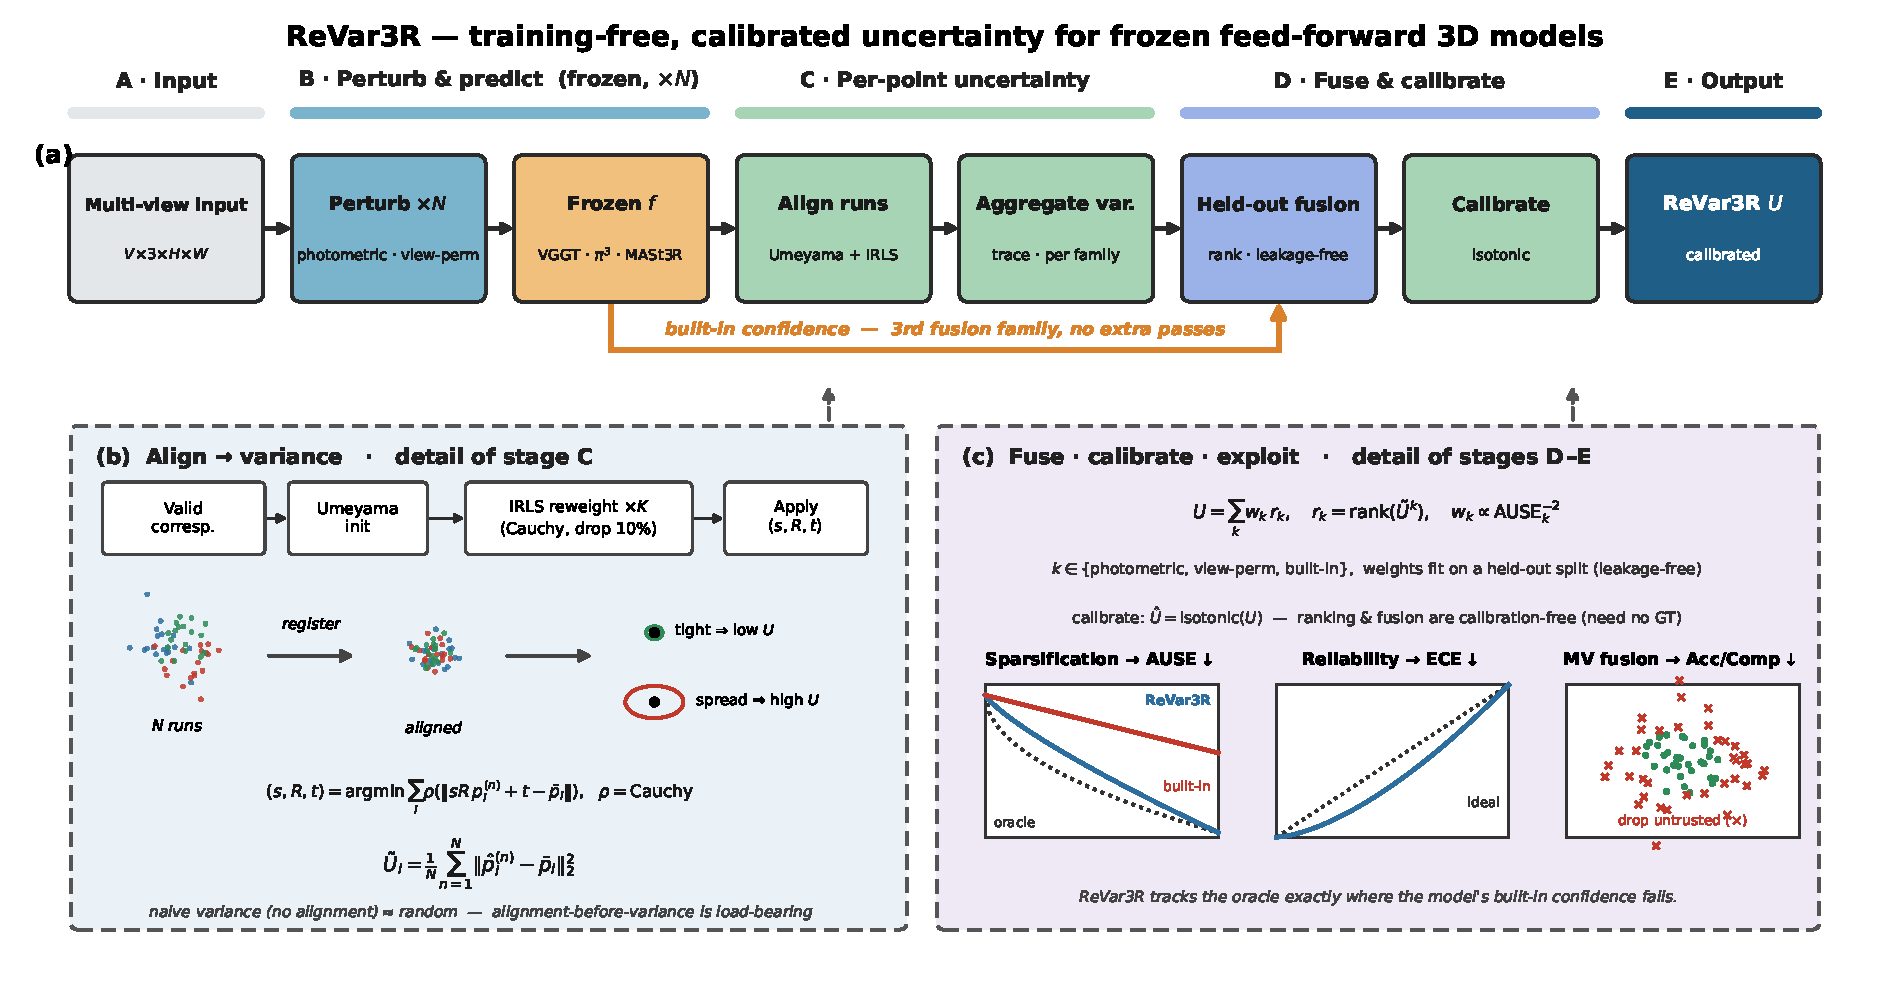
\includegraphics[width=\textwidth]{pipeline.pdf}
  \caption{\textbf{\trustr\ overview.} \emph{When the model's own confidence lies, perturbation
  tells the truth.} (a) The training-free pipeline: run the \emph{frozen} model $N$ times under
  geometry-preserving perturbations, robustly align each run into a common frame, take per-point
  trace-variance, fuse the two perturbation families \emph{together with} the model's own built-in
  confidence via held-out, leakage-free weights, and calibrate. (b) The alignment-before-variance step (our technical crux), with the
  robust-alignment and trace-variance equations. (c) The held-out fusion and isotonic-calibration
  equations, and how the uncertainty $U$ is evaluated and exploited downstream.}
  \label{fig:pipeline}
\end{figure*}

These models do emit a per-pixel \emph{confidence}, but it is trained as a reconstruction
loss-weight, not a calibrated uncertainty---the 3D analogue of softmax mis-calibration~\cite{guo}.
A 2025 survey~\cite{survey3d} explicitly names uncertainty quantification for this model family
\emph{``critical and underexplored.''} We give the first systematic evidence of how unevenly the
built-in confidence behaves: it is weak in-distribution---near-random for some model/dataset pairs
(VGGT/7-Scenes Spearman $+0.07$)---and \textbf{collapses where reliability matters most}: its
correlation with error falls to $\approx0$ out-of-distribution (ETH3D, all three models) and turns
\emph{negative} on several in-distribution cells (VGGT/BlendedMVS $-0.12$, MASt3R/DTU $-0.10$). A
signal that flat-lines or inverts under the very shift where reliability matters is worse than useless.

We propose \trustr, a \emph{training-free} estimator that obtains a calibrated per-point
uncertainty from a \emph{frozen} model by measuring its \emph{disagreement with itself} under
small, geometry-preserving input perturbations (photometric jitter and input-view
permutation/subsetting). The key technical subtlety, absent in 2D test-time-augmentation
uncertainty~\cite{ayhan,ttaaleatoric}, is that each perturbed run expresses geometry in its own
gauge: we therefore \emph{robustly register every run into a common frame before measuring
variance} (Umeyama~\cite{umeyama} + IRLS), then take per-point trace-variance, isotonic-calibrate,
and fuse the two estimators by held-out rank-weighting. The estimator needs $\le 10$ forward
passes and runs on a single 16\,GB GPU.

Across \vggt, \pii\ and \mastr\ on four datasets (7-Scenes, DTU, BlendedMVS, ETH3D), \trustr\
significantly reduces \ause\ in \textbf{9 of 12} model$\times$dataset cells (by $3\text{--}36\%$,
paired Wilcoxon)---\emph{including the OOD set for all three architectures, where the built-in
confidence collapses}. The wins are \emph{predicted} by where the confidence is mis-calibrated and
the non-wins are exactly the BlendedMVS cells (the models' training corpus, where the confidence is
already well-calibrated)---a mechanistic coupling, not blanket superiority.
Strikingly, \trustr\ matches or beats an MLP \emph{trained} on the model's own frozen features,
which tells us the usable reliability signal is \emph{epistemic input-sensitivity}, only visible
when the model is actually re-run, rather than a static function of one forward pass. We make the
following contributions:

\begin{itemize}[leftmargin=1.2em,itemsep=1pt,topsep=2pt]
\item \textbf{C1 (a failure mode, characterized).} The first systematic evidence that the built-in
confidence of frozen 3D foundation models is an \emph{uneven} uncertainty---weak in-distribution and
\emph{collapsing} ($\rho{\approx}0$) or \emph{anti-correlated} ($\rho<0$) where reliability matters
most---across three models and four datasets (\Cref{sec:rq1}).
\item \textbf{C2 (alignment-before-variance).} A training-free estimator whose crux is robust
similarity registration of each perturbed run before per-point variance. This is not an engineering
detail but the conceptual core: in 3D each run expresses geometry in its own gauge, so \emph{naive}
perturbation variance is near-random ($0.72$ vs.\ $0.50$ \ause)---registration is what turns
self-disagreement into a usable signal, and the ablation shows it is the single largest contributor
(\Cref{sec:method,sec:exp}).
\item \textbf{C3 (the epistemic insight).} \trustr\ matches/beats a probe trained on the model's
frozen features, evidence that the signal is epistemic input-sensitivity, not in the static
features (\Cref{sec:exp}).
\item \textbf{C4 (a calibrated benchmark + utility).} A reproducible single-GPU protocol
(\ause/\aurg/Spearman/\ece\ + fused-cloud Accuracy/Completeness), a near-oracle multi-view-fusion
utility, and \emph{honest negatives} (no NVS gain; a falsified architectural hypothesis).
\end{itemize}

\noindent\textbf{Paper organization.} \Cref{sec:questions} states the research questions, hypotheses,
and novelty; \Cref{sec:primer} fixes background and notation; \Cref{sec:rq1} documents the
confidence-collapse failure mode; \Cref{sec:method} develops the method; \Cref{sec:exp} and
\Cref{sec:ablations} present the results and ablations; and \Cref{sec:discussion} discusses scope and
limitations.
